\documentclass[]{book}
\usepackage{lmodern}
\usepackage{amssymb,amsmath}
\usepackage{ifxetex,ifluatex}
\usepackage{fixltx2e} % provides \textsubscript
\ifnum 0\ifxetex 1\fi\ifluatex 1\fi=0 % if pdftex
  \usepackage[T1]{fontenc}
  \usepackage[utf8]{inputenc}
\else % if luatex or xelatex
  \ifxetex
    \usepackage{mathspec}
  \else
    \usepackage{fontspec}
  \fi
  \defaultfontfeatures{Ligatures=TeX,Scale=MatchLowercase}
\fi
% use upquote if available, for straight quotes in verbatim environments
\IfFileExists{upquote.sty}{\usepackage{upquote}}{}
% use microtype if available
\IfFileExists{microtype.sty}{%
\usepackage{microtype}
\UseMicrotypeSet[protrusion]{basicmath} % disable protrusion for tt fonts
}{}
\usepackage[margin=1in]{geometry}
\usepackage{hyperref}
\hypersetup{unicode=true,
            pdftitle={R for Psych Handbook},
            pdfauthor={David John Baker},
            pdfborder={0 0 0},
            breaklinks=true}
\urlstyle{same}  % don't use monospace font for urls
\usepackage{natbib}
\bibliographystyle{apalike}
\usepackage{color}
\usepackage{fancyvrb}
\newcommand{\VerbBar}{|}
\newcommand{\VERB}{\Verb[commandchars=\\\{\}]}
\DefineVerbatimEnvironment{Highlighting}{Verbatim}{commandchars=\\\{\}}
% Add ',fontsize=\small' for more characters per line
\usepackage{framed}
\definecolor{shadecolor}{RGB}{248,248,248}
\newenvironment{Shaded}{\begin{snugshade}}{\end{snugshade}}
\newcommand{\KeywordTok}[1]{\textcolor[rgb]{0.13,0.29,0.53}{\textbf{#1}}}
\newcommand{\DataTypeTok}[1]{\textcolor[rgb]{0.13,0.29,0.53}{#1}}
\newcommand{\DecValTok}[1]{\textcolor[rgb]{0.00,0.00,0.81}{#1}}
\newcommand{\BaseNTok}[1]{\textcolor[rgb]{0.00,0.00,0.81}{#1}}
\newcommand{\FloatTok}[1]{\textcolor[rgb]{0.00,0.00,0.81}{#1}}
\newcommand{\ConstantTok}[1]{\textcolor[rgb]{0.00,0.00,0.00}{#1}}
\newcommand{\CharTok}[1]{\textcolor[rgb]{0.31,0.60,0.02}{#1}}
\newcommand{\SpecialCharTok}[1]{\textcolor[rgb]{0.00,0.00,0.00}{#1}}
\newcommand{\StringTok}[1]{\textcolor[rgb]{0.31,0.60,0.02}{#1}}
\newcommand{\VerbatimStringTok}[1]{\textcolor[rgb]{0.31,0.60,0.02}{#1}}
\newcommand{\SpecialStringTok}[1]{\textcolor[rgb]{0.31,0.60,0.02}{#1}}
\newcommand{\ImportTok}[1]{#1}
\newcommand{\CommentTok}[1]{\textcolor[rgb]{0.56,0.35,0.01}{\textit{#1}}}
\newcommand{\DocumentationTok}[1]{\textcolor[rgb]{0.56,0.35,0.01}{\textbf{\textit{#1}}}}
\newcommand{\AnnotationTok}[1]{\textcolor[rgb]{0.56,0.35,0.01}{\textbf{\textit{#1}}}}
\newcommand{\CommentVarTok}[1]{\textcolor[rgb]{0.56,0.35,0.01}{\textbf{\textit{#1}}}}
\newcommand{\OtherTok}[1]{\textcolor[rgb]{0.56,0.35,0.01}{#1}}
\newcommand{\FunctionTok}[1]{\textcolor[rgb]{0.00,0.00,0.00}{#1}}
\newcommand{\VariableTok}[1]{\textcolor[rgb]{0.00,0.00,0.00}{#1}}
\newcommand{\ControlFlowTok}[1]{\textcolor[rgb]{0.13,0.29,0.53}{\textbf{#1}}}
\newcommand{\OperatorTok}[1]{\textcolor[rgb]{0.81,0.36,0.00}{\textbf{#1}}}
\newcommand{\BuiltInTok}[1]{#1}
\newcommand{\ExtensionTok}[1]{#1}
\newcommand{\PreprocessorTok}[1]{\textcolor[rgb]{0.56,0.35,0.01}{\textit{#1}}}
\newcommand{\AttributeTok}[1]{\textcolor[rgb]{0.77,0.63,0.00}{#1}}
\newcommand{\RegionMarkerTok}[1]{#1}
\newcommand{\InformationTok}[1]{\textcolor[rgb]{0.56,0.35,0.01}{\textbf{\textit{#1}}}}
\newcommand{\WarningTok}[1]{\textcolor[rgb]{0.56,0.35,0.01}{\textbf{\textit{#1}}}}
\newcommand{\AlertTok}[1]{\textcolor[rgb]{0.94,0.16,0.16}{#1}}
\newcommand{\ErrorTok}[1]{\textcolor[rgb]{0.64,0.00,0.00}{\textbf{#1}}}
\newcommand{\NormalTok}[1]{#1}
\usepackage{longtable,booktabs}
\usepackage{graphicx,grffile}
\makeatletter
\def\maxwidth{\ifdim\Gin@nat@width>\linewidth\linewidth\else\Gin@nat@width\fi}
\def\maxheight{\ifdim\Gin@nat@height>\textheight\textheight\else\Gin@nat@height\fi}
\makeatother
% Scale images if necessary, so that they will not overflow the page
% margins by default, and it is still possible to overwrite the defaults
% using explicit options in \includegraphics[width, height, ...]{}
\setkeys{Gin}{width=\maxwidth,height=\maxheight,keepaspectratio}
\IfFileExists{parskip.sty}{%
\usepackage{parskip}
}{% else
\setlength{\parindent}{0pt}
\setlength{\parskip}{6pt plus 2pt minus 1pt}
}
\setlength{\emergencystretch}{3em}  % prevent overfull lines
\providecommand{\tightlist}{%
  \setlength{\itemsep}{0pt}\setlength{\parskip}{0pt}}
\setcounter{secnumdepth}{5}
% Redefines (sub)paragraphs to behave more like sections
\ifx\paragraph\undefined\else
\let\oldparagraph\paragraph
\renewcommand{\paragraph}[1]{\oldparagraph{#1}\mbox{}}
\fi
\ifx\subparagraph\undefined\else
\let\oldsubparagraph\subparagraph
\renewcommand{\subparagraph}[1]{\oldsubparagraph{#1}\mbox{}}
\fi

%%% Use protect on footnotes to avoid problems with footnotes in titles
\let\rmarkdownfootnote\footnote%
\def\footnote{\protect\rmarkdownfootnote}

%%% Change title format to be more compact
\usepackage{titling}

% Create subtitle command for use in maketitle
\newcommand{\subtitle}[1]{
  \posttitle{
    \begin{center}\large#1\end{center}
    }
}

\setlength{\droptitle}{-2em}
  \title{R for Psych Handbook}
  \pretitle{\vspace{\droptitle}\centering\huge}
  \posttitle{\par}
  \author{David John Baker}
  \preauthor{\centering\large\emph}
  \postauthor{\par}
  \predate{\centering\large\emph}
  \postdate{\par}
  \date{2018-03-22}

\usepackage{booktabs}
\usepackage{amsthm}
\makeatletter
\def\thm@space@setup{%
  \thm@preskip=8pt plus 2pt minus 4pt
  \thm@postskip=\thm@preskip
}
\makeatother

\usepackage{amsthm}
\newtheorem{theorem}{Theorem}[chapter]
\newtheorem{lemma}{Lemma}[chapter]
\theoremstyle{definition}
\newtheorem{definition}{Definition}[chapter]
\newtheorem{corollary}{Corollary}[chapter]
\newtheorem{proposition}{Proposition}[chapter]
\theoremstyle{definition}
\newtheorem{example}{Example}[chapter]
\theoremstyle{definition}
\newtheorem{exercise}{Exercise}[chapter]
\theoremstyle{remark}
\newtheorem*{remark}{Remark}
\newtheorem*{solution}{Solution}
\begin{document}
\maketitle

{
\setcounter{tocdepth}{1}
\tableofcontents
}
\chapter{Preface}\label{preface}

This book serves as a collection of resources used in the LSU
psychological statistics courses. It contains some lecture notes, as
well as R code and data to run each of the examples in R.

The book is still under construction.

\chapter{Introduction to R}\label{intro}

You can label chapter and section titles using \texttt{\{\#label\}}
after them, e.g., we can reference Chapter \ref{intro}. If you do not
manually label them, there will be automatic labels anyway, e.g.,
Chapter \ref{methods}.

Figures and tables with captions will be placed in \texttt{figure} and
\texttt{table} environments, respectively.

\begin{Shaded}
\begin{Highlighting}[]
\KeywordTok{par}\NormalTok{(}\DataTypeTok{mar =} \KeywordTok{c}\NormalTok{(}\DecValTok{4}\NormalTok{, }\DecValTok{4}\NormalTok{, .}\DecValTok{1}\NormalTok{, .}\DecValTok{1}\NormalTok{))}
\KeywordTok{plot}\NormalTok{(pressure, }\DataTypeTok{type =} \StringTok{'b'}\NormalTok{, }\DataTypeTok{pch =} \DecValTok{19}\NormalTok{)}
\end{Highlighting}
\end{Shaded}

\begin{figure}

{\centering 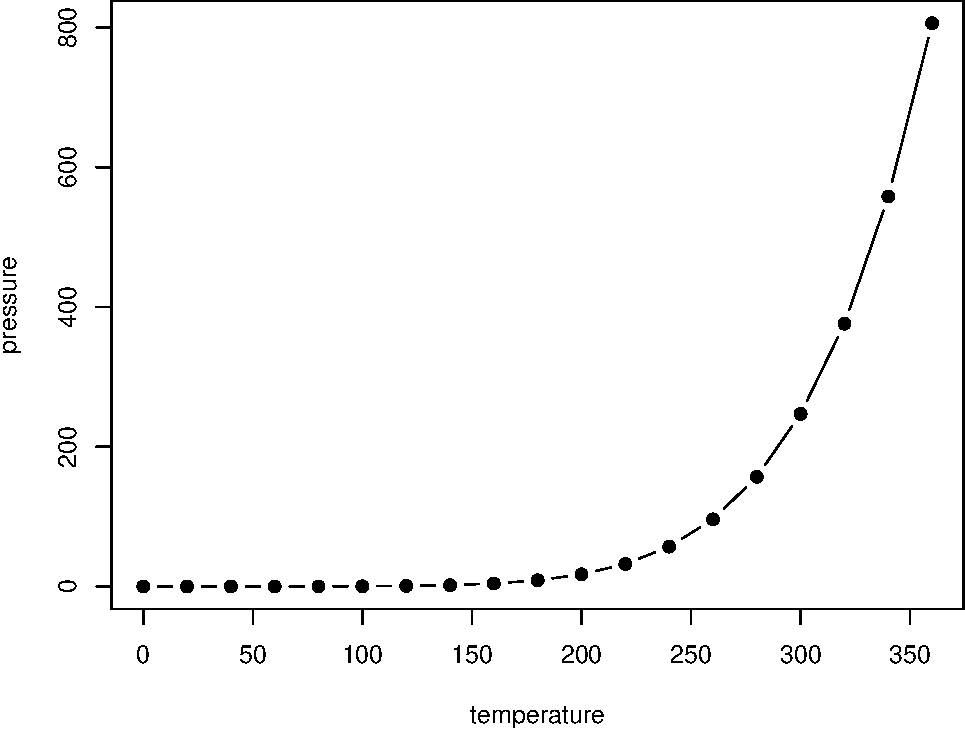
\includegraphics[width=0.8\linewidth]{bookdown-demo_files/figure-latex/nice-fig-1} 

}

\caption{Here is a nice figure!}\label{fig:nice-fig}
\end{figure}

Reference a figure by its code chunk label with the \texttt{fig:}
prefix, e.g., see Figure \ref{fig:nice-fig}. Similarly, you can
reference tables generated from \texttt{knitr::kable()}, e.g., see Table
\ref{tab:nice-tab}.

\begin{Shaded}
\begin{Highlighting}[]
\NormalTok{knitr}\OperatorTok{::}\KeywordTok{kable}\NormalTok{(}
  \KeywordTok{head}\NormalTok{(iris, }\DecValTok{20}\NormalTok{), }\DataTypeTok{caption =} \StringTok{'Here is a nice table!'}\NormalTok{,}
  \DataTypeTok{booktabs =} \OtherTok{TRUE}
\NormalTok{)}
\end{Highlighting}
\end{Shaded}

\begin{table}

\caption{\label{tab:nice-tab}Here is a nice table!}
\centering
\begin{tabular}[t]{rrrrl}
\toprule
Sepal.Length & Sepal.Width & Petal.Length & Petal.Width & Species\\
\midrule
5.1 & 3.5 & 1.4 & 0.2 & setosa\\
4.9 & 3.0 & 1.4 & 0.2 & setosa\\
4.7 & 3.2 & 1.3 & 0.2 & setosa\\
4.6 & 3.1 & 1.5 & 0.2 & setosa\\
5.0 & 3.6 & 1.4 & 0.2 & setosa\\
\addlinespace
5.4 & 3.9 & 1.7 & 0.4 & setosa\\
4.6 & 3.4 & 1.4 & 0.3 & setosa\\
5.0 & 3.4 & 1.5 & 0.2 & setosa\\
4.4 & 2.9 & 1.4 & 0.2 & setosa\\
4.9 & 3.1 & 1.5 & 0.1 & setosa\\
\addlinespace
5.4 & 3.7 & 1.5 & 0.2 & setosa\\
4.8 & 3.4 & 1.6 & 0.2 & setosa\\
4.8 & 3.0 & 1.4 & 0.1 & setosa\\
4.3 & 3.0 & 1.1 & 0.1 & setosa\\
5.8 & 4.0 & 1.2 & 0.2 & setosa\\
\addlinespace
5.7 & 4.4 & 1.5 & 0.4 & setosa\\
5.4 & 3.9 & 1.3 & 0.4 & setosa\\
5.1 & 3.5 & 1.4 & 0.3 & setosa\\
5.7 & 3.8 & 1.7 & 0.3 & setosa\\
5.1 & 3.8 & 1.5 & 0.3 & setosa\\
\bottomrule
\end{tabular}
\end{table}

You can write citations, too. For example, we are using the
\textbf{bookdown} package \citep{R-bookdown} in this sample book, which
was built on top of R Markdown and \textbf{knitr} \citep{xie2015}.

\chapter{Data Manipulation in R}\label{data-manipulation-in-r}

Here is a review of existing methods.

\chapter{Episotomology of Statistics}\label{episotomology-of-statistics}

We describe our methods in this chapter.

\chapter{Descriptive Statistics, z Scores, Central
Limit}\label{descriptive-statistics-z-scores-central-limit}

Some \emph{significant} applications are demonstrated in this chapter.

\section{Example one}\label{example-one}

\section{Example two}\label{example-two}

\chapter{Data Transformations and Confidence
Intervals}\label{data-transformations-and-confidence-intervals}

We have finished a nice book.

\chapter{Power and Effect Size
Measures}\label{power-and-effect-size-measures}

attempt here

\chapter{Correlation and Regression}\label{correlation-and-regression}

attempt here

\chapter{Matched T Test}\label{matched-t-test}

Template file

\chapter{One Way ANOVA}\label{one-way-anova}

Template file

\chapter{Multiple Comparisons}\label{multiple-comparisons}

Template file

\chapter{Simple Effects, Interactions, Mixed
Designs}\label{simple-effects-interactions-mixed-designs}

Template file

\chapter{Repeated Measures ANOVA:}\label{repeated-measures-anova}

Template file

\chapter{Mixed Two Way ANOVA}\label{mixed-two-way-anova}

Template file

\chapter{Multiple Regression}\label{multiple-regression}

Template file

\chapter{Chi-Square}\label{chi-square}

Template file

\chapter{Non-Parametric Data}\label{non-parametric-data}

Template file

\chapter{Advanced Data Cleaning}\label{advanced-data-cleaning}

Template file

\chapter{Advanced Multiple
Regression}\label{advanced-multiple-regression}

Template file

\chapter{Logistic Regression}\label{logistic-regression}

Template file

\chapter{Mediation and Moderation}\label{mediation-and-moderation}

Template file

\chapter{ANCOVA}\label{ancova}

\section{Theory}\label{theory}

\subsection{Reducing Noise}\label{reducing-noise}

Just like the ANOVA (Analysis of Variance), the ANCOVA (Analysis of
Covariance) is used to analyze experiments by calculating an F ratio for
more than 2 groups. As with any F calculation, differences in the
dependent variable are caused by two things:

\begin{enumerate}
\def\labelenumi{\arabic{enumi}.}
\tightlist
\item
  The independent variable (signal, systematic variation)
\item
  Error (noise, unsysematic variation)
\end{enumerate}

The F statistic captures this

\[ F = \frac{Variation\ Due\ to\ IV}{Variation\ Due\ to\ Error} \]

When there is small variation within groups and large variation between
groups, we get a large F.

CHART HERE

When there is large variatin within groups and small variation between
groups, we get a small F.

The idea with the ANCOVA is that you can reduce your error term (the
denominator from above) by choosing a covariate (CV) that is related to
the DV and will soak up some random variation in your F test to give you
a clearer picture of what is going on. Usually this means controlling
for some sort of variable. The classic example is if you wanted to give
some kids a test of some mental ability in a between subjects design but
you don't want their age to skew your results. You might have had a
control condition, an intervention, and some sort of alternate
intervention. Typically you would run an ANOVA on the three groups, but
since you know age has been accounted for and you want to remove that
effect from the model, you enter age as a covariate in this calculation.
Outside of this there are \textbf{three} major applications for ANCOVA.

\begin{enumerate}
\def\labelenumi{\arabic{enumi}.}
\tightlist
\item
  Increase test sensitivity by using the CV(s) to account for more of
  the error variance
\item
  Adjust DV scores to what they would be if everyone scored the same on
  the CV(s)
\item
  Adjustment of a DV for other DVs taken as CVs
\end{enumerate}

Note that use of a CV can adjust DV scores and show a larger effect or
the CV can even eliminate the effect. Looking at this another way:

\begin{enumerate}
\def\labelenumi{\arabic{enumi}.}
\tightlist
\item
  Reduces random error by increasing the size of F
\item
  Reduces systematic error by adjusting for differences in means
\item
  May increase differences by soaking up error
\end{enumerate}

It's a \textbf{good} idea to use ANCOVA when you are removing variance
in the DV related to covariate, but not related to the grouping
variable. This decreases the error term and increases power.

It'sa \textbf{bad} idea to use ANCOVA when groups differ on their mean
level of the covariate. Usually here the covariate and the grouping
variable are not independent. An example of this might be when
``controlling'' for anxiety when studying people with and without
depression. Clearly people with depression will have higher levels of
anxiety than their controls by nature of having depression!

\subsection{Assumptions of ANOVA}\label{assumptions-of-anova}

\begin{enumerate}
\def\labelenumi{\arabic{enumi}.}
\tightlist
\item
  All ANOVA assumptions apply (errors are RIND)
\end{enumerate}

\begin{itemize}
\tightlist
\item
  Random
\item
  Independent
\item
  Normally distributed
\end{itemize}

\begin{enumerate}
\def\labelenumi{\arabic{enumi}.}
\setcounter{enumi}{1}
\tightlist
\item
  The Covariate z is unrelated to x, and that z is related to, and in a
  sense, acts as a suppressor of y
\item
  The covariate has a \textbf{linear} relationship with the dependent
  variable
\item
  Variance of groups are equal.
\item
  Correlation between y and z is equal for all levels of x (Homogeneity
  of Regression)
\end{enumerate}

You test for homogeneity of regression slopes by including a covariate
by group interaction. If it's significant, you violated an assumption
and can't to ANCOVA!

CHART

CHART

\subsection{Best Practice}\label{best-practice}

Things you should control for: 1. Broad Descriptors (Age, Social Class)
2. General Ability (intellgience, memory, speed of movement) 3.
Personality measures (extraversion, neuroticism) 4. Things you think are
relevant 5. Pick CVs that are correlated with DV * Height good for
basketball * Height poor for test of math skills 6. CV should not be
influenced by treatment

\section{Practice}\label{practice}

In order to get our hands dirty with ANCOVA we're going to look at a
dataset where a bunch of sheep were slaughtered. We have three types of
sheep (ewe, wether, ram) and a measure of fatness and weight.

Let's first run an ANOVA to see if fatness differs between animal type.

\begin{Shaded}
\begin{Highlighting}[]
\KeywordTok{library}\NormalTok{(data.table)}
\NormalTok{deadsheep <-}\StringTok{ }\KeywordTok{fread}\NormalTok{(}\StringTok{"datasets/deadsheep.csv"}\NormalTok{)}
\NormalTok{deadsheep[, Animal }\OperatorTok{:}\ErrorTok{=}\StringTok{ }\KeywordTok{as.factor}\NormalTok{(animal)]}
\NormalTok{sheep.model.}\DecValTok{1}\NormalTok{ <-}\StringTok{ }\KeywordTok{aov}\NormalTok{(fatness }\OperatorTok{~}\StringTok{ }\NormalTok{Animal, }\DataTypeTok{data=}\NormalTok{deadsheep)}
\KeywordTok{summary}\NormalTok{(sheep.model.}\DecValTok{1}\NormalTok{)}
\end{Highlighting}
\end{Shaded}

\begin{verbatim}
##             Df Sum Sq Mean Sq F value Pr(>F)  
## Animal       2  124.4   62.21   3.165 0.0566 .
## Residuals   30  589.6   19.65                 
## ---
## Signif. codes:  0 '***' 0.001 '**' 0.01 '*' 0.05 '.' 0.1 ' ' 1
\end{verbatim}

Looking at the output, we note that There was no significant effect of
fatness on levels of animal, \[F(2,30)=3.165, p > .05\].

Now since we know that the whole weight of the animal might be
confounding our answer (it's related to the DV of fatness, but not
nessecarily related to the type of sheep), let's run an ANCOVA with
carcass weight as a covariate and see if that changes our answer.

Before we run the ANCOVA, we need to first check that our IV is not
significantly related to our CV. We do this by running an ANOVA
predicting weigth by animal.

\begin{Shaded}
\begin{Highlighting}[]
\CommentTok{#Test IND of IV and CV}
\NormalTok{ind.sheep <-}\StringTok{ }\KeywordTok{aov}\NormalTok{(weight }\OperatorTok{~}\StringTok{ }\NormalTok{Animal, }\DataTypeTok{data=}\NormalTok{deadsheep) ## Check CV for IV indep, want non-sig}
\KeywordTok{summary}\NormalTok{(ind.sheep) }\CommentTok{# p=.104}
\end{Highlighting}
\end{Shaded}

\begin{verbatim}
##             Df Sum Sq Mean Sq F value Pr(>F)
## Animal       2  14.20   7.102   2.438  0.104
## Residuals   30  87.41   2.914
\end{verbatim}

Here we get\[ F(2,30) = 2.44, p> .05\] and can move forward. Let's now
run our ANCOVA. Note that R's default is Type I Sum of Squares, we need
to load the \texttt{car} package to give us the correct sum of squares.
For further reading on this, check out the Andy Field book on this.

\begin{Shaded}
\begin{Highlighting}[]
\NormalTok{sheepANCOVA <-}\StringTok{ }\KeywordTok{aov}\NormalTok{(fatness }\OperatorTok{~}\StringTok{ }\NormalTok{Animal }\OperatorTok{+}\StringTok{ }\NormalTok{weight, }\DataTypeTok{data=}\NormalTok{deadsheep)}
\KeywordTok{library}\NormalTok{(car)}
\KeywordTok{Anova}\NormalTok{(sheepANCOVA, }\DataTypeTok{type=}\StringTok{"III"}\NormalTok{)}
\end{Highlighting}
\end{Shaded}

\begin{verbatim}
## Anova Table (Type III tests)
## 
## Response: fatness
##             Sum Sq Df F value    Pr(>F)    
## (Intercept) 117.17  1  26.529 1.669e-05 ***
## Animal      332.31  2  37.621 8.772e-09 ***
## weight      461.56  1 104.506 3.994e-11 ***
## Residuals   128.08 29                      
## ---
## Signif. codes:  0 '***' 0.001 '**' 0.01 '*' 0.05 '.' 0.1 ' ' 1
\end{verbatim}

We can then report

The covariate, weight, was not significantly related to the the fatness
of the animal, \[F(1, 29) =,p=.0565 \] and that there was a significant
effect of the animal after controlling for weight of the animal,
\[F(2,28) = 37.62, p < .05.\].

Let's now check on our marginal means. These are our group means after
we have controlled for our covariate. For this we need the
\texttt{effects} package.

\begin{Shaded}
\begin{Highlighting}[]
\KeywordTok{library}\NormalTok{(effects)}
\NormalTok{mean.sheep <-}\StringTok{ }\KeywordTok{effect}\NormalTok{(}\StringTok{"Animal"}\NormalTok{, sheepANCOVA, }\DataTypeTok{se=}\OtherTok{TRUE}\NormalTok{)}
\KeywordTok{summary}\NormalTok{(mean.sheep)}
\end{Highlighting}
\end{Shaded}

\begin{verbatim}
## 
##  Animal effect
## Animal
##      Ewe      Ram   Wether 
## 18.90219 10.53996 14.83058 
## 
##  Lower 95 Percent Confidence Limits
## Animal
##       Ewe       Ram    Wether 
## 17.565871  9.183322 13.532447 
## 
##  Upper 95 Percent Confidence Limits
## Animal
##      Ewe      Ram   Wether 
## 20.23851 11.89660 16.12870
\end{verbatim}

We can then note the estimated marginal means here (18.9 for Ewe, 10.53
for Ram, and 14.83 for Wether) are mean values for fatness once the CV
of weight has been controlled for.

Lastly, let's test the homogenaity of the regression slopes assumption
(though we should have done this first!). We do this by running the
model with an interaction term included.

\begin{Shaded}
\begin{Highlighting}[]
\NormalTok{hoRS.sheep <-}\StringTok{ }\KeywordTok{aov}\NormalTok{(fatness }\OperatorTok{~}\StringTok{ }\NormalTok{weight }\OperatorTok{+}\StringTok{ }\NormalTok{Animal }\OperatorTok{+}\StringTok{ }\NormalTok{animal}\OperatorTok{:}\NormalTok{weight, }\DataTypeTok{data=}\NormalTok{deadsheep)}
\KeywordTok{Anova}\NormalTok{(hoRS.sheep, }\DataTypeTok{type=}\StringTok{"III"}\NormalTok{)}
\end{Highlighting}
\end{Shaded}

\begin{verbatim}
## Anova Table (Type III tests)
## 
## Response: fatness
##                Sum Sq Df F value    Pr(>F)    
## (Intercept)    64.571  1 14.6355 0.0007007 ***
## weight        180.144  1 40.8308 7.624e-07 ***
## Animal          5.293  2  0.5998 0.5560672    
## weight:animal   8.957  2  1.0151 0.3757923    
## Residuals     119.123 27                      
## ---
## Signif. codes:  0 '***' 0.001 '**' 0.01 '*' 0.05 '.' 0.1 ' ' 1
\end{verbatim}

The interaction term is not significant, thus no violation. We can also
plot this to see it. All regression lines should be pointing in the same
direction when we plot the groups separately.

\begin{Shaded}
\begin{Highlighting}[]
\KeywordTok{library}\NormalTok{(ggplot2)}
\KeywordTok{ggplot}\NormalTok{(deadsheep, }\KeywordTok{aes}\NormalTok{(}\DataTypeTok{x =}\NormalTok{ weight, }\DataTypeTok{y =}\NormalTok{ fatness, }\DataTypeTok{color =}\NormalTok{ Animal)) }\OperatorTok{+}\StringTok{ }
\StringTok{  }\KeywordTok{geom_point}\NormalTok{() }\OperatorTok{+}\StringTok{ }
\StringTok{  }\KeywordTok{geom_smooth}\NormalTok{(}\DataTypeTok{method =} \StringTok{"lm"}\NormalTok{) }\OperatorTok{+}\StringTok{ }
\StringTok{  }\KeywordTok{labs}\NormalTok{(}\DataTypeTok{title =} \StringTok{"Homogeneity of Regression Slopes"}\NormalTok{, }\DataTypeTok{x =} \StringTok{"Weight"}\NormalTok{, }\DataTypeTok{y =} \StringTok{"Fatness"}\NormalTok{)}
\end{Highlighting}
\end{Shaded}

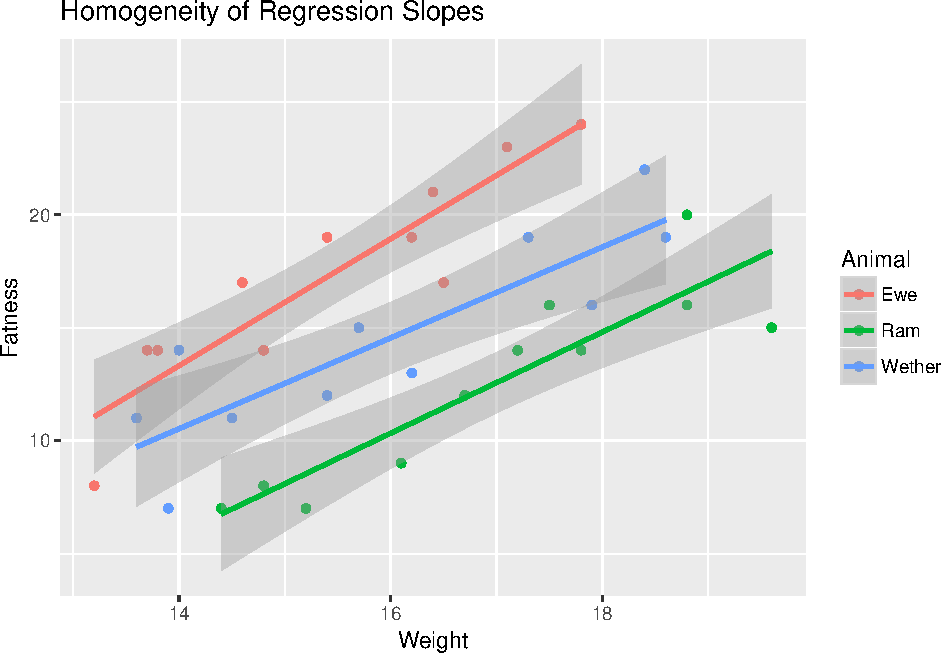
\includegraphics{bookdown-demo_files/figure-latex/unnamed-chunk-6-1.pdf}

If one of these lines would be pointed downwards, we would have an
interaction.

\chapter{MANOVA}\label{manova}

Template file

\chapter{Repeated Measures ANOVA}\label{repeated-measures-anova-1}

Template file

\chapter{Factor Analysis}\label{factor-analysis}

Template file

\chapter{Mixed Effects Models}\label{mixed-effects-models}

Template file

\chapter{Confirmatory Factor
Analysis}\label{confirmatory-factor-analysis}

Template file

\chapter{This is a template file}\label{this-is-a-template-file}

Template file

\bibliography{packages.bib,book.bib}


\end{document}
